\documentclass{acm_proc_article-sp}
\usepackage{biblatex}
\bibliography{biblio}
\bibliography{Papers/SECURWARE/securware}
\bibliography{imc}
\bibliography{Papers/ESORICS/esorics.bib}
%\usepackage[backend=biber,style=numeric]{biblatex}
%\addbibresource{biblio.bib}
%\addbibresource{Papers/SECURWARE/securware.bib}
%\addbibresource{Papers/IMC -  Internet Measurement Conference/imc.bib}
%\addbibresource{Papers/ESORICS/esorics.bib}
%Note: ‘ ’ in the final document should be changed to plain apostrophes '
% Also “ ” should be replaced by plain quotation marks "
%\tolerance=1000 % force latex to be a bit more generous with hyphenation and line breaking?

\begin{document}

\title{Investigating the Security Features of Botnets}
\subtitle{CPSC 526 Final Report \\ Tutorial Section: T02}
\date{\today}
\numberofauthors{3}
\author{
\alignauthor
Stephen Dixon\\
       \email{sjdixon2@gmail.com}
\alignauthor
Kevin Chum\\
       \email{kchum@gmail.com}
\alignauthor
Rafael Benicio\\
       \email{rafaelbenicio2@gmail.com}
}

\maketitle

\begin{abstract}

In this paper, we investigate how the security and functionality of botnets are achieved by examining how botnet features are implemented, throughout each stage of the bot program.

At the infection stage, botnets employ a number of means to circumvent security mechanisms, such as anti-anti-virus, exploitation frameworks, and polymorphic engines.  In addition, bot programs usually check for the presence of debuggers, virtualization software, and other contextual factors which could indicate that the environment is a honeypot.  A number of mechanisms exist to prevent reverse-engineering of the binary program as well, such as code that decompresses and decrypts itself as it executes.

Botnets are typically organized in a hybridized peer-to-peer structure with some central components.  Command and control is maintained through structured network topologies and digital signatures.  Network resilience is made possible through a number of security mechanisms designed to protect against sinkholing and partitioning attacks.  Some of these security mechanisms include guards against node injection and sinkhole announcements; others include fallback modes which reinitialize binaries and configuration files in the event that the node remains static.


\end{abstract}
\category{D3.3}{Operating System}{Security Protection}[Invasive Software]
\terms{Security}
\keywords{Malware, botnets, network security}

\newpage
\section{Introduction}

Malware is one of the most serious threats facing the internet today, as it provides miscreants the means to perform a wide range of illegal and damaging activities, including distributed denial of service attacks, click fraud, data theft, and spam. According to McAfee and the Center for Strategic and International Studies, global cyber crime activity costs the world economy an estimated amount between \$300 billion and \$1 trillion dollars every year \cite{lewis:economics}.

Arguably, the most common form of malware today are bots; bots are programs which link compromised machines together in a command-and-control (C\&C) network; such networks, called botnets, allow botmasters to control and coordinate the bots by uploading payloads \cite{jacob:infiltration}.  Botnets used for a variety of purposes, such as fraud, theft, espionage, phishing, spam, and distributed denial of service attacks.

Botnets can be created in a variety of ways.  Some malware providers offer pay-per-installation services to help botmasters spread their programs \cite{caballero:distribution}.  Botnets can also be created through the use of a malicious proxy server which injects javascript code into web content using a man-in-the-middle attack; so-called javascript botnets are able to reach large audiences quickly and cheaply, but with reduced capability, as the malicious code is stored in the browser cache \cite{defcon:javascript}.

Botnets can communicate using a variety of channels.  Some botnets communicate over plain text, whereas other botnets employ their own proprietary cryptographic protocols to securely communicate between nodes \cite{stone:takeover}.  Botnets communicating to their botmasters via voice-over-IP (VOIP) have also been proposed \cite{defcon:voip} as well.  

Contemporary network security researchers have noticed that botnets are rapidly migrating from centralized server-based networks to peer-to-peer networks.\cite{botnet:history}  The reason for this migration is that peer-to-peer networks are more resilient against takeover, reconnaissance, and remediation efforts.  However, researchers have noted that most peer-to-peer botnets are actually hybrids \cite{defcon:prowling}, as botmasters still rely on centralized servers in order to collect the data collected by their bots.  Typically, such botnets consist of a modest number of relay nodes which serve as conduits between the central server and leaf nodes; many nodes, however, are actually unreachable by the botnet because they are located behind NAT networks, and must initiate contact with the bot server on their own. 

By establishing a systematic understanding of how botnets are structured and implemented, we can effectively challenge their influence. Despite the diversity of botnets on the internet, they often share similar purposes, and therefore share common challenges and design tradeoffs.  On a fundamental level, botnets depend on communication between mutually untrusted parties\cite{stone:p2p}, and often they depend on some central components, despite the movement towards peer-to-peer protocols.


\section{Objectives}

Generally speaking, botnets conform to the analogy of a bank robbery: first, the robbers must penetrate their target (through subtle force or trickery), and then they must make a clean getaway with the stolen goods. In phishing scams, the purpose of the botnet is to spread word about a scam to unsuspecting victims. Typically, the victims are tricked into purchasing objects like viagra, drugs, pills, or stock, or into giving away personal information or credit card information; these transactions are then exploited to defraud or rob the victims of their money
\cite{defcon:javascript}
\cite{defcon:spam}
\cite{wikipedia:phishing}.  On the other hand, botnets that use trojan-horses like Zeus collect sensitive information from victims by injecting web content into otherwise secure websites, keylogging, and remote access\cite{defcon:javascript}
\cite{blackhat:zeus}
\cite{defcon:spam}
\cite{wikipedia:trojan}. In most schemes, information and commands are exchanged between the harvester bots (which collect information) and the botmaster through an impure peer-to-peer network through the use of relay nodes and proxy servers. Innovative schemes, such as the VOIP botnet proposed by Itzik Kotler et. al of Security Art, would improve on the traditional botnet model by eliminating the need to exfiltrate data to a central server\cite{defcon:voip}.

Our objective in this paper is to explain the way in which bot programs are implemented, with the hope that future development can address each of the weaknesses they rely on for their continued existence.  In this paper, we examine features across all stages of the bot program, as implemented by real botnets such as Zeus and ZeroAccess.

First, we analyze how machines are infected, and how they are recruited into the botnet. Second, we analyze various mechanisms used by bot programs in order to circumvent security  and frustrate reverse-engineering. Thirdly, we examine various strategies for implementing command and control protocols which can be used by the botmaster to carry out the purposes of the botnet. Fourthly, we investigated several ways in which harvester bots can exfiltrate data anonymously and securely to the botmaster.  Finally, we investigated the peer-to-peer networking protocols implemented by various botnets, and how they respond to sinkholing attacks.  In each of these sections, we focus on the features of the botnet and how they lend themselves to the survival and prosperity of the botnet.

By botnet features, we mean any protocol, algorithm, or process implemented by a bot program which realizes the purpose of the botnet.  Depending on the purpose of the botnet, bot programs may vary substantially.  For example, the Zeus botnet uses trojan horses in order to steal and use financial information from its victims; consequently, it requires the ability to collect the information harvested by bots.  As a result of this, it is designed around a number of central components which in turn relay the harvested information to a rapidly changing group of command and control systems. One of Zeus' features is that, if a bot finds that it has been isolated from the network, or if it remains static for too long, it will automatically compute the address of the control server and reinitialize.

An important limitation of this paper is that the purpose, design, and implementation of criminal botnets are intentionally kept secret by their authors; consequently, we are limited to information which is publicly known. However, in some lucky cases, botnet authors do not implement secure features or protocols. Our sources include academic conferences such as USENIX, ACSAC,  and CCS, as well as black-hat conferences such as DEFCON.  

%Centralized
%Major Driver: Control
%Major Weakness: Resilience

\section{How Infection is Implemented}
% How Bots Get Infected
    %- how systems get infected

There are several widely known infection mechanisms for bots.  For example, attackers can scan a target subnet for known vulnerabilities and infect victims through exploitation and penetration tools\cite{feily:detection}.  Attackers can also employ social engineering methods in order to trick users into downloading and executing malicious executables; in the past, email attachments and html code were used, but this has gone out of favour as many email services such as Gmail now block executable attachments.

Another method of infection is through drive-by-downloads.  Drive-by-downloads are downloads which occur without the informed consent of the victims; often, the user thinks they are downloading one application, but in fact, there are unwanted programs bundled with it. A number of potentially unwanted programs are known to be installed this way, such as the Conduit search bar.

A final vector of approach is through cross-site scripting.  Cross-site scripting attacks allow attackers to inject executable code into the user browsers, which is then executed by the victims.  The main drawback of cross-site scripting attacks is that they persist only while the user's browser is active, unlike penetration-based or download-based infection, which grant the attacker full access to the Windows platform. However, cross-site scripting can still be used for botnet creation, as an attacker can use the javascript to download malicious payloads from the bot server\cite{defcon:javascript}.

After installation, the attacker must then disable the security systems on the target machine. Security can be bypassed and deactivated in a number of a ways, including polymorphic engines, as discussed in the next section. Once security is disabled, the attacker can then download payload programs from other sites through the use of shell code.  These payload programs allow attackers to install a portfolio of malware on to the target machine, including the bot programs for it to participate in botnets.  The bot program itself is essentially a bundle of malware containing modules for command-and-control, data theft, backdoor access, botnet propagation, and more.

\subsection{Avoiding Detection by Antiviruses}
Because the main method through which botnets propagate is by malicious code, they must have methods to thwart anti-virus utilities. Otherwise they would be detected and rendered unable to infect a target machine. 

In the event that a protected computer does manage to become infected and join the botnet --- for example, if the strain of malware has not yet been detected by security companies --- then the malware may be able to kill any antivirus process that might be running, and block access to the vendor's website \cite{barford:book}. This might be done by editing the HOSTS file on Windows machines, or through the interception of packets being sent from or received by the infected machine. For botnets that have become widely known in the industry, this method becomes unfeasible without more sophisticated tactics.

The key weakness in most antivirus tools is that they work by comparing scanned binaries to a list of known malware signatures. However, malware signatures are typically unknown for newly released malware. As a result, botnet creators can take advantage of this property by writing malware that does not have a consistent signature. For example, the Storm botnet had multiple variants with different signatures that were released at certain intervals in order to circumvent antivirus scanning. By applying this principle on a large scale, botnet creators are able to easily stay ahead of antivirus updates. This technique is also known as \emph{serial variant evasion} \cite{ollmann:evasion}. There are several ways that new signatures can be generated, and these methods can be combined together to make an even larger set of possible signatures.

Metamorphic code (and also polymorphic code) is one method through which botnets can avoid antiviruses. The virus changes the 'look' of the binary without changing the semantics and overall meaning. This can be done, for example by exchanging two instructions where order does not matter, or by changing way the code achieves its purpose: using different registers or using different instructions to achieve the same thing. For instance in x86 assembly code, the instruction \texttt{xor eax eax} is syntactically different but causes the same end result as \texttt{mov eax 0}. Malware employ this method during propagation in order to have a different looking signature at each infection, thus circumventing any signature-based antivirus detection.

Another way to change the signature of malicious code is to add redundant or useless data, known as noise. This can be done either in the actual code of the malware or in its binary. In the code, a malware author can include constructs that essentially do nothing, for example testing if $1=1$, performing an arithmetic calculation without saving the result in a variable, or adding NOPs. They can also write functions or add variables that are not actually used by the program. One last method is to add code routines that logically will not occur. For noise insertion to binaries, the programmer can add (possibly non-interpretable) data to the beginning or the end of the binary. Usually the malicious code itself is not modified. This insertion of garbage also has the added benefit that the malware producer can expand the malicious file to any arbitrary size that is desired, for example to match the filesize of some known benign file that is shared publicly, say in a torrent.

One more method that allows for changing virus signatures is to change how the compiler works on the code. Different compilers, versions of compilers, and settings used in compilation can drastically change how the final binary appears. In fact, some malware vendors utilize some automation frameworks like scripts to automatically change compilation variables \cite{ollmann:evasion}. However there is a caveat with this method: there are only so many ways to tweak settings in order to produce a new binary. Thus this method is not often seen on its own and instead combined with other techniques.


    % avoiding reverse engineering by sniffers, debuggers, honeypots etc.
\subsection{Avoiding Reverse Engineering by Sniffers, Debuggers, and Honeypots}

Most of the aforementioned techniques provide protection at the code level. That is, they do not directly manipulate the binary after it has been created, with the exception of noise injection. There are several techniques that are used to generate new signatures by changing the binary in some way instead, and are used widely by malware. However, more importantly these techniques also provide protection against reverse engineering.

Even when the malware manages to evade antivirus detection and convert some machine into a bot, it cannot be considered safe. Rather, it might be in a hostile environment and at the scrutiny of researchers and security experts hoping to glean information from the running process or binary. In order to prevent this, malware must provide some way to prevent against procedures like reverse engineering and capture by these individuals. Many of the techniques that are utilized originated as ways to provide copyright protection and have since been adapted for use in malware \cite{ollmann:evasion}.

Some kinds of malware employ encryption to provide protection from signature detection and static analysis of the binary. The contents of the malicious code are encrypted and, upon being executed, are decrypted as the program runs. This makes it difficult for virus scanners to search for predefined regular expressions of known malicious strings. Additionally, debugging tools are unable to perform their analyses without proper knowledge of the decryption algorithm and key.

Another method that is widely used by malware is compression. Tools known as \emph{packers} exist that shrink the size of binaries to be more portable across slow Internet connections. However these tools are also used by malware to make it more difficult for antiviruses to detect the malicious code contained in the binary. For example, the packer UPX is a popular executable compression utility used both commercially and by malware. There are also some packers that allow for polymorphic output: the binary appears structurally different on each execution of the packed executable. Thus direct disassembly is prevented as the debugger is unable to complete its analysis of the code. This can be circumvented, however it requires more effort when trying to reverse engineer the malware.

There are also tools known as \emph{binders} that attempt to embed malware into legitimate-looking software. This helps promote the spread of malware (and thus the botnet) by tricking users into executing the malicious binary and become infected.

In addition to these methods, malware can directly scan for the presence of debuggers, breakpoints, and virtualization software in their code. The Honeynet project outlines some of the ways this is achieved and also provides source code of these techniques, written in assembly \cite{honeynet:appendix}. These checks include tests for popular debugging tools such as SoftICE and OllyDbg, as well as tests for breakpoints in general. There is also a test that verifies the presence of VMware by executing certain backdoor function calls. After a test returns true, there are several options available to malware. In the event that a debugger is detected, it can attempt to kill the debugger or jump to code that does something different from what it usually does, in order to deter reverse engineers. For virtualization and sandbox software, malware could attempt to exploit vulnerabilities in the code in order to 'jump out' of the sandbox and infect the host computer. Alternatively, the malware could shut itself down, thereby frustrating the efforts of researchers trying to use it on a virtual environment.

All of these techniques can be used together, and in fact, are bundled together into a single program called a protector. One such piece of software is the RDG Tejon Crypter, which provides anti-debuggers, anti-virtualization, anti-anti-virus, and binder capabilities\cite{rdg:crypter}. 

Another facet of botnets that is probed by researchers is the communication protocol between bots and the command server, if any. Methods to protect against this include using proprietary protocols and encryption. However, there are botnet detection techniques that can detect botnet communication even past encryption \cite{feily:detection}. Some data-mining and DNS-based detection techniques are also able to find botnets regardless of their protocol and structure \cite{gu:botminer}. This technique is effective even if the command and control structure and protocol of a botnet changes. In addition, some researchers have devised automated methods to reverse-engineer botnet protocols and detection \cite{freiling:tracking} \cite{caballero:dispatcher} \cite{gu:botsniffer}. 

\section{How Command and Control is Implemented}
% Evolution of Command & Control
    % single point of access (admin console)
    % communication channels for propagating commands/updates
% IRC, HTTP, HTTPS, encryption
% gossip protocols
% minimizing traffic footprint
% unreachable nodes
    % execution of commands?


When creating botnets, one major design decision lies in how bots are connected to each other and to the botmaster. The network topology plays a major role in determining how botmasters exert control over their botnets, collect harvested data, and update bot programs. As of the time of writing, there are two major ways that botnets can be structured: as a centralized command and control (C\&C) infrastructure, or as a distributed peer-to-peer (P2P) network.  Most botnets today rely on hybrids of both categories, in order to combine the dominance of central servers and the resilience of peer-to-peer networks\cite{stone:p2p}\cite{defcon:prowling}.

In a centralized command and control scheme, there is some central server from which a botmaster can control and update bots. Individual bots can also send any obtained data to this server, in the case that the botnet's malicious payload includes spyware. Centralized command and control structures are attractive due to the fact that there is a single point of access for a botmaster, for instance through some web browser-based admin console. Through this point, they can command botnets to download new payloads, launch certain attacks or scans, or propagate on their network. For example, the Zeus botnet comes with a browser-based control panel, where botmasters can send new rules to, or collect data from bots. Using this application, they can also group different bots together and name them individually \cite{blackhat:zeus}. Command and control protocols may use Internet Relay Chat (IRC), or message gossiping schemes implemented through HTTP and peer-to-peer networking.  In the Asprox network, HTTP is the primary protocol used to communicate between botmasters and bots\cite{borgaonkar:analysis}. 

Of the botnets that use IRC, Rajab et al. noted in 2006  \cite{rajab:botnets} that there were four prominent substructures. The first is the simplest and most widely used, where all bots connect to a single chat server. This structure has the disadvantage that the server capacity was often reached. To combat this problem and to support larger botnets, another structure is used where multiple IRC servers are linked together to form a network that has higher capacities. These botnets are known as \emph{bridged botnets}. Another method that is used by botmasters is to have several botnets that appear distinct but can be deduced to (via analysis of naming conventions and user IDs) be likely to belong to the same botmaster. The final observed structure is one where a subset of bots in one server are made to download a new binary that moves them to a different server. Commands in an IRC-based botnet are typically made by setting the channel topic to some string recognized by the bots to be a command \cite{honeynet:appendix}, whereas in an HTTP-based botnet, bots regulalry poll a C\&C web server while waiting for new commands to be received \cite{borgaonkar:analysis}.

Due to the prominence of IRC as a method for botnets to communicate, many corporations block ports related to the protocol, or carefully monitor IRC traffic. As such, current trends in botnet communication appears to indicate a move towards more commonly seen protocols such as HTTP, and towards P2P networks \cite{cooke:survey}.


HTTP is often combined with peer-to-peer networking in a \emph{gossip protocol}. This kind of protocol relies on nodes passing on information that is learned to other nodes, thereby propagating it throughout the network. Gossip protocols are employed by peer-to-peer botnets \cite{defcon:prowling}, but can be utilized by hierarchical command and control botnets as well. Due to the need for communication to spread by nodes, the propagation speed is usually slower than direct messaging. However in larger botnets, this reduces the strain on the central C\&C server by delegating the command passing to other bots; it also has the effect of diffusing traffic throughout the botnet, thereby improving the network's overall resilience and reducing the likelihood that the botnet will be detected.

Ollmann et. al classified gossip-based C\&C botnets into several topological groups\cite{ollmann:topology}, some of which appear to have counterparts to the IRC substructures. One of these is called the \emph{Star topology}. In this setup, each bot communicates directly with a single, centralized C\&C server. Another topology, similar to the idea of bridged botnets, is the multi-server C\&C topology. As the name implies, this method introduces several servers that act as command and control servers to the botnet. In a hierarchical topology, bots are organized in a hierarchy, and bots that are higher up in the hierarchy can issue commands to bots further down in the tree.

\section{How Data is Exfiltrated from Harvester Bots}
%Evolution of Collection/Anonymity (the getaway car)
%    - anonymity (tor, proxy servers, voip)
%    - location (fast flux, voip)
%    - how is communication different when sending info back to server?

Once data has been collected by bots, the process of exfiltrating the data back to the botmaster for monetization begins.  For some botnets, communication with the botmaster occurs before data exfiltration.  In this section, we describe several of the methods bots use to communicate with the botmaster without exposing the identity of the bot server.

The most common method of communicating with the botmaster is to use anonymizing proxy servers.  Proxy servers are middlemen that forward requests from one client to a server on the other end.  When a bot wants to send a request to the botmaster, it relays the encrypted request through the anonymizing proxy server; an adversary sniffing the headers of the requests on either side of the proxy will not be able to map the client to the server.  However, the reliability of this channel depends on the trustworthiness and availability of the proxy servers used by the botnet.  Botnets may account for availability by selecting one out of many botnets for traffic, and they may account for potential tampering by using multiple proxy servers, onion routing, and message validation\cite{stone:p2p}\cite{defcon:prowling}.

There are several alternative methods as well. Several botnets, such as Mevade (also known as LazyAlienBikers), have attempted to use Tor, a well-known anonymity network.  Tor anonymizes traffic between two endpoints through the use of onion routing and random paths.   However, the Tor network collects metrics, meaning that the botnet risks exposure as a result of using the service. The Mevade botnet was virtually undiscovered before it started using Tor; however, after switching to the network, specialists from the security firm Damballa were able to track, analyze, and disrupt the botnet\cite{damballa:tor}. 

The reason for the attention on this botnet was due to the sudden increase in traffic within the Tor network after Mevade changed their communication methods \cite{darkreading:tor}. Evidently botnets risk detection if they cause too much suspicious network traffic, and so should have design considerations to that end. Most botnets are programmed so that an individual bot does not perform any actions without instructions from the botmaster\cite{honeynet:appendix}. 

As another example of minimizing suspicious traffic, a commercial botnet was developed to buy cars included error validation functions\cite{defcon:cars}. This functionality was added to avoid an IP ban from server administrators; had there been no error validation, the server administrators could’ve potentially noticed that a large amount of invalid traffic was being generated from a single IP address.

Recently, researchers identified the potential for VOIP-based botnets.  VOIP, or voice over IP, is a protocol used for performing phone and conference calls over the internet.  A VOIP-based botnet could leverage any unused conference call numbers in order to exfiltrate data by phone.  By using digital-tone multi-frequency signalling as a means of encoding and decoding between binary and sound, hackers would be utilize the channel in the same way that IP uses bytes.  In addition to providing the botmaster with an anonymous form of communication, VOIP botnets:

\begin{itemize}
\item can be operated from a payphone or mobile
\item can be accessed from the phone network and the internet
\item are not blocked by typical IDS/IPS signatures
\item leverage a channel which is significantly harder to monitor
\end{itemize}

No botnets are known to use VOIP yet.  However, according to recent reports, the Sality botnet is known to have scanned all IPv4 addresses in search of vulnerable VOIP servers\cite{sality:scan}.


\section{How Peer-to-Peer Networking Is Implemented}

Contemporary botnets like ZeroAccess, MinerBot, Zeus, and Storm have adopted hybridized network structures in an effort to combine the resilience of peer-to-peer networks with the controllability of centralized servers\cite{defcon:prowling}.  Centralized servers are easy to construct, but have a single point of weakness: the command and control server itself \cite{wang:p2p}.  The nature of the network topology is surprisingly similar between peer-to-peer botnets;  ~\ref{fig:p2p-architecture} outlines the topology of peer-to-peer networks found in the likes of botnets such as ZeroAccess, MinerBot, Zeus, Storm, Conficker, and Kelihos.

\begin{figure}[ht]\centering
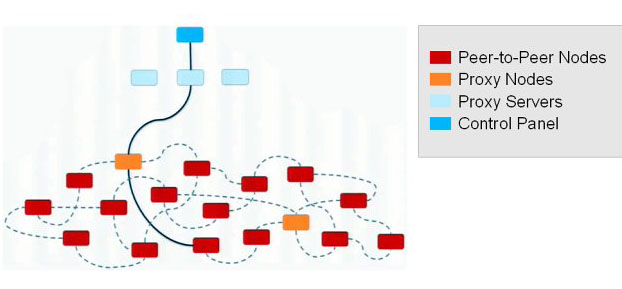
\includegraphics[width=0.47\textwidth,natheight=640,natwidth=340]{p2p-architecture.jpg}
\caption{Peer-to-Peer Botnet Topology}
\label{fig:p2p-architecture}
\end{figure}

In these botnets, when individual bots want to receive commands from the botmaster, they send a request to some central components, through the use of peers, proxy nodes, and proxy servers. There is usually a layer of proxy servers being used, in order to provide redundancy in case they are taken down. Relaying requests in this manner helps disguise the location of the bot server on the internet \cite{defcon:prowling}.

Individual bots maintain a list of peers, obtained by communicating with other bots in the network.  In the ZeroAccess protocol, the peer list consists of a list of IP addresses and a timestamp indicating how recently the bot was active; the list was sorted in order of how recently the bot was active. In version 1 of the protocol, the peer list was 256 bots long and would bots that have not been active recently; in version 2, the peer list is 16 bots long and showed bots only if they were active recently.  It was suggested that the length of the peer lists were trimmed in order to reduce the traffic footprint of the botnet, as the botnet grew in size  \cite{defcon:prowling}.  

However, not all bots in the peer list are reachable.  Bots can be unreachable for a variety of reasons, such as being located inside NAT networks, or due to IP address churn.   Consequently, P2P botnets rely extensively on nodes which can be reached from anywhere; these nodes form the backbone of the botnet because of their positioning \cite{defcon:prowling}.

Message gossiping is utilized to propagate information\cite{stone:p2p}. A gossip protocol is a protocol in which a bot, in response to receiving information from another bot, forwards it to their peers. Each botnet uses customized message types and gossip protocols. For example, the Zeus botnet has the following message types:\cite{zeus:protocol}
\begin{itemize}
\item version request and reply - to determine a bot's current binary and configuration file\cite{zeus:protocol}.
\item peer list request and reply - to determine who the bot communicates with\cite{zeus:protocol}.
\item data request and reply - used to pull updates to the Zeus bot's binary or configuration files via UDP\cite{zeus:protocol}.
\item Proxy Reply - a signed message containing a list of proxies returned sent in response to a version request with some piggybacked proxy request markers\cite{zeus:protocol}.
\item Proxy Announcement - a message announcing that a bot has been appointed as a proxy by the botmasters.  This message is then forwarded to the peer list of the bots who received the message.  To minimize the traffic footprint, this message type includes a time-to-live field which is decremented each time the message is forwarded; after reaching 0, bots do not forward the announcement any further\cite{zeus:protocol}.
\item C2 Message Type - a specialized, encrypted message exchanged between harvester bots and proxies, exchanged over HTTP and TCP protocols.  C2 message requests are sent by harvester bots to inform the server of the type of information harvested by the bot; the reply allows Zeus to tell the bot what to do with the information \cite{zeus:protocol}.
\end{itemize}

\subsection{Techniques for Reconnaissance and Disruption}
%\subsection{Reconnaissance and Disruption Techniques} %This one doesn't hyphenate for some reason leaving some overhanging words and an overfull hbox

Research into peer-to-peer botnets has yielded a number of useful techniques for reconnaissance and disruption.  Reconnaissance is aimed at determining the size, topology, and vulnerabilities of a botnet, whereas disruption techniques are aimed at shutting down the botnets for good.  Two common reconnaissance techniques are crawling and sensor injection.  Crawling techniques use the peer-list mechanism implemented by botnets to determine all peers within the network, and who they are connected to. A number of factors limit the accuracy of crawling techniques; these include IP churn, non-routable peer clusters, peers with multiple IP addresses, and the frequency with which bots communicate with other bots.  Sensor injection techniques count the number of peers in a botnet by using the researcher's own machine as a relay node; this has the same effect as crawling does, except that some previously unreachable nodes will communicate with the sensor node.  In both reconnaissance techniques, a final approximate figure for the size of the botnet is obtained when the number of bots counted by the crawler or sensor converges towards a specific value \cite{stone:p2p}\cite{defcon:prowling}.

Common disruption techniques include sinkholing (in which bots are redirected to an offensive machine called a sinkhole) and partitioning (which aims to split the botnet into unusable subnets) \cite{stone:p2p}.  A sinkholing attack consists of several steps:
\begin{itemize}
\item Sinkhole Announcement - the intended sinkhole is sent to as many peers as possible.
\item Node isolation - the attacker attempts to eliminate all edges in the P2P graph that do not point to the sinkhole, effectively isolating peers from each other.
\item Fallback Prevention - many botnets have mechanisms that allow the bots to communicate directly with the command and control center in the event of a sinkhole attack.  Attackers must somehow disable the fallback channel or prevent bots from entering their fallback mode.
\end{itemize}

Botnets in the wild have employed a number of defenses against sinkhole attacks.  For example, the Sality botnet uses a reputation scheme in which each bot keeps track of the reputation of its neighbouring peers; reputation is increased by correctly responding to requests, and decreased by incorrectly responding to requests. Peers shared their peer lists only with other machines with high reputation, and only allow peer list entries with low reputations to be overwritten. Stone Gross et. al reverse-engineered the protocol to the extent that they could create their own high-reputation node, and they found ways to poison existing high-reputation nodes by overwriting their port numbers \cite{stone:p2p}.

On the other hand, the Zeus network uses a different scheme to prevent and mitigate sinkholing. Zeus bots announce their presence by sending requests to other bots on their peer list; upon receiving a request, Zeus bots add the source to its peer list if it knows fewer than 50 peers.  Zeus accounts for IP churn by assigning unique IDs to each bot, and updating the IP address whenever it receives an update for the bot identified with an ID it knows about.  Zeus mitigates the effect of spoofing through the use of an automated IP-based blacklist, which blocks IP addresses with high request rates \cite{stone:p2p}.

Furthermore, botnets employ a wide variety of fallback mechanisms in the wild.  Zeus bots periodically verify their neighbours every few days; if the bot is unable to update itself or its configuration files for seven days, it attempts to obtain a fresh peer list by contacting a set of hardcoded IP addresses, or by using a domain generation algorithm to lookup an appropriate command and control server.  As a result of these mechanism, sinkholing operations against Zeus are only temporarily successful \cite{stone:p2p}.

Domain generation algorithms, also known as domain flux and fast flux, grant bots the ability to communicate directly with the central components of a botnet.  However, the critical issue with domain generation algorithms is that the botnet reverts back to a centralized, non-P2P network, meaning that, once again, the network's resilience depends on how long these central resources can last.  In the case of the Torpig botnet, researchers were able to reverse-engineer the fast flux algorithm and take control of the botnet for over ten days\cite{stone:takeover}.  In the case of the Zeus network, the domain generation algorithm has recently been decrypted by a group of researchers; it is possible that, given the predictability of the algorithm, that the domains may be blocked by internet providers before they can be used as a fallback channel\cite{zeus:protocol}.


\subsection{Mathematical Underpinning of Botnets}

Researchers have proposed a variety of metrics for quantitatively measuring the robustness and efficiency of botnets.  Both attributes matter from a security perspective: efficient botnets produce less traffic, and therefore go undetected for longer.  The robustness of the network, on the other hand, is the major aim of peer-to-peer network structures such as those implemented for botnets such as Zeus and ZeroAccess.  Botnets routinely gain and lose new members over time; a higher degree of connections between bots provides fault tolerance and recovery, as well as resilience against attacks such as sinkholing\cite{botnet:metrics}.  Dagon et. al proposed a number of metrics for measuring the robustness of a botnet, such as the following:

\begin{itemize}
\item inverse geodesic distance (a normalized measurement which reflects the overall connectivity of the botnet network topology)
\item the network diameter (which measures the average geodesic length between two nodes in a network)
\item a clustering coefficient to measure the local transitivity (ie. the likelihood that three nodes appear in a "triad") in a neighborhood of peers.
\end{itemize}

However, it does not appear that these metrics have been collected for contemporary botnets.

\section{Conclusion}

Contemporary botnets are highly sophisticated peer-to-peer networks with some central components, and are frequently equipped with fallback mechanisms to ensure their resilience against takedown and infiltration attempts.  Botmasters employ a wide range of means in order to achieve infection, download the payload bot program, and disable security systems on the compromised machine.

For infections based on social engineering and drive-by-downloads, malware authors can bypass the security offered by anti-virus programs by using polymorphic engines, which scramble the binary code of the application in such a way as to make a bot program unrecognizable to the anti-virus.  In order to prevent the bot program from being reverse-engineered by researchers, malware authors have employed a variety of schemes, including features which detect the presence of virtualization services and debuggers.

After infection is achieved, the bot is ready to join the botnet.  The challenge faced by botnets is to make it easy to join, but hard to infiltrate.  The advantage enjoyed by researchers is that botnets depend upon the communication of mutually untrustworthy parties\cite{stone:p2p}. In order to guard the botnet against infiltration and sinkholing attempts, botnets have employed a variety of different security mechanisms. 

In the Sality botnet, bots implement a reputation scheme in which they internally track the reputation of each of their peers, and overwrite low-reputation entries in their peer list.  However, researchers have been able to bypass the scheme by reverse-engineering the protocol in order to create a high-reputation bot; as a result, they were able to poison high-reputation entries and sinkhole other components of the network.

In the Zeus network, sinkhole protection is provided by ensuring that bots have a limited number of peers, and by promoting the retention of peer lists.  These effectively limit the effects of change to the network, thereby boosting the resiliency of the botnet.  Furthermore, even if the botnet could be taken down, there are a number of fallback mechanisms that allow peers to re-establish themselves by communicating with some central components.

Meanwhile, in terms of their capacity, botnets continue to be a growing threat.  Command and control consoles provide a single point of access to botmasters to administer thousands of compromised machines at the click of a mouse.  Usage of P2P technologies improve the resilience of botnets, but so far, most botnets continue to use some central components to maintain their hold on the control infrastructure. Innovations like VOIP-based botnets provide botmasters a means of reaching new and hitherto unreachable networks without the need for a central server, while exploiting a common, readily available channel which is much more difficult to inspect or protect\cite{defcon:voip}.  Their effect has yet to be seen.

\printbibliography{}

\end{document}
